\section{Question 2}

X is a discrete-valued random variable with uniform distribution over the set $\{-2, -1, 0, 1, 2\}$. 
Draw its probability mass function (PMF) and calculate $\E[X]$ and $\var[X]$.

\noindent\rule{\textwidth}{.5pt}

Let $p:\mathbb{Z} \to \mathbb{R}$ denote the PMF of $X$.
Since the random variable is uniform on $\{x\in\mathbb{Z}: |x|<3\}$, we have
%
\begin{equation}
    p(x) = \begin{cases}
        k, & |x| < 3 \\ 
        0, & |x| \geq 3
    \end{cases}
\end{equation} 
%
for some constant $k>0$.
Since the PMF must satisfy the identity $\sum_{x \in \mathbb{Z}} p(x) = 1$, we have 
%
\begin{align}
    \sum_{x \in \mathbb{Z}} p(x) = 
    \sum_{|x| \geq 3} p(x) + 
    \sum_{|x| < 3} p(x) &= 1 \\
    0 + 5k &= 1 \quad\therefore\quad k = \frac{1}{5}
\end{align}

The drawing in \cref{fig:pmf} illustrates the PMF with $k$ evaluated. 
%
\begin{figure}[htbp]
    \centering
    \caption{PMF of an uniform distribution in $\{-2, -1, 0, 1, 2\}.$}
    \label{fig:pmf}
    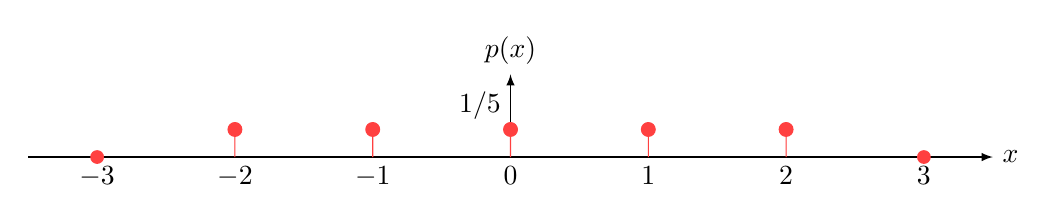
\begin{tikzpicture}[> = latex, scale=1.75]
    \def\r{0.05}
    % Axis
    \draw [->] (-3.5, 0) -- (3.5, 0) node [right] {$x$};
    \draw [->] (0, 0) -- (0, 0.6) node [above] {$p(x)$};
    \draw (0, 0.2) node [above left] {$1/5$};
    % Curve
    \foreach \x in {-2, -1, 0, 1, 2}{
        \draw (\x, 0) node [below] {$\x$};
        \draw [red!75, fill=red!75] (\x, 0) --++ (0, 0.2) circle (\r);
    }
    \fill [red!75] (-3, 0) circle (\r);
    \fill [red!75] (3, 0) circle (\r);
    \draw
        (-3, 0) node [below] {$-3$}
        (3, 0) node [below] {$3$};

\end{tikzpicture}
\end{figure}
%
As for $\E[X]$ and $\var[X]$, we can use the definition for the $n$-th moment 
$\E[X^n] = \sum_{x\in\mathbb{Z}} x^n p(x)$ and the definition 
$\var[X] = \E[(X - \E[X])^2] = \E[X^2] - \E[X]^2$:
%
\begin{align}
    \E[X] 
    &= \sum_{|x|<3} \frac{x}{5}
    = \frac{1}{5}(-2-1+0+1+2)
    = 0 
    \\
    \E[X^2]
    &= \sum_{|x|<3} \frac{x^2}{5}
    = \frac{1}{5}[(-2)^2 + (-1)^2 + 0^2 + 1^2 + 2^2]
    = 2
    \\
    \var[X] 
    &= \E[X^2] - \E[X]^2
    = 2 - 0
    = 2
\end{align}